\documentclass{beamer}
%%%%%%%%%%%%%%%%%%%%%%%%%%%%%%%%%%%%%%%%%%%%%%%%%%%%%%%%%%%%%%%%%%%%%%%%%%%%
\usepackage{bm}
\usepackage{amsmath}
\usepackage{amssymb}
%\usepackage{microtype}
\usepackage{booktabs} % \toprule, \midrule, \bottomrule
/Users/seth/Documents/Compositions/SRJinclude.tex
\newcommand{\Dtens}{\mat{D}}
\definecolor{lightgray}{gray}{0.85}
\newcommand{\notebox}[1]{\hspace{.1\columnwidth}\colorbox{lightgray}{\parbox{0.8\columnwidth}{\small
#1}}}
\newcommand{\epsiloncolor}[1]{\textcolor{blue}{#1}}
%%%%%%%%%%%%%%%%%%%%%%%%%%%%%%%%%%%%%%%%%%%%%%%%%%%%%%%%%%%%%%%%%%%%%%%%%%%%

\usetheme{AnnArbor}
\usecolortheme{seahorse}
\usecolortheme{orchid}
\usefonttheme[onlymath]{serif}
\setbeamercolor*{frametitle}{use=structure,bg=structure.fg!20!white}
\setbeamercolor*{frametitle right}{use=structure,bg=structure.fg!20!white}
\setbeamertemplate{navigation symbols}{\insertframenavigationsymbol}
\setbeamertemplate{caption}[numbered]

\title[Prospectus]%
{A Physics-Based Anisotropic Diffusion Method for Thermal Radiative
Transfer}
%\subtitle{}

\author[Seth~R.~Johnson]{Seth~R.~Johnson (and EWL?)}

\institute[UMich]{
University of Michigan, Ann Arbor
}
\date[11/3/2010]{November 3, 2010}

%\AtBeginSection[]
%{
%\begin{frame}
%  \frametitle{Outline}
%  \tableofcontents[currentsection]
%\end{frame}
%}
%
\hypersetup{colorlinks=true,linkcolor=black}

% only show section headings in table of contents
\setcounter{tocdepth}{1}

%use symbols for footnote
\renewcommand{\thefootnote}{\fnsymbol{footnote}}

\begin{document}
%%%%%%%%%%%%%%%%%%%%%%%%%%%%%%%%%%%%%%%%%%%%%%%%%%%%%%%%%%%%%%%%%%%%%%%%%%%%

\begin{frame}
\titlepage
\begin{center}
  \includegraphics[width=0.2\textwidth]{../figures/umlogo}
\end{center}
\end{frame}

%%%%%%%%%%%%%%%%%%%%%%%%%%%%%%%%%%%%%%%%%%%%%%%%%%%%%%%%%%%%%%%%%%%%%%%%%%%%
\section{Introduction}
%%%%%%%%%%%%%%%%%%%%%%%%%%%%%%%%%%%%%%%%
\begin{frame}
  \frametitle{Thermal radiative transfer}
  Radiation $T^4$ is the dominant heat transfer process

  Applications in high energy density physics:
  \begin{itemize}
    \item Stellar astrophysics, strategic astrophysics
    \item Inertial confinement fusion
    \item CRASH (Center for RAdiative Shock Hydrodynamics) program: ``Assessment
          of Predictive Capability''
  \end{itemize}
  Difficulties in solving:
  \begin{itemize}
    \item High dimensionality of solution phase space $(\vec{x}, \vec{\Omega},
      h\nu, t)$
    \item Highly nonlinear coupled partial differential equations for radiation
      field $I(\vec{x}, \vec{\Omega}, h\nu, t)$ and material energy $U_m(\vec{x}, t)$
  \end{itemize}
\end{frame}
%%%%%%%%%%%%%%%%%%%%%%%%%%%%%%%%%%%%%%%%
\begin{frame}
  \frametitle{Motivation}
\begin{center}
  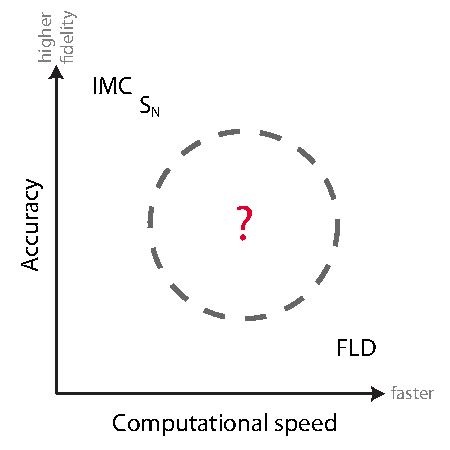
\includegraphics[width=3in]{../figures/fidelity}
\end{center}
% also, storage requirements
\end{frame}
%%%%%%%%%%%%%%%%%%%%%%%%%%%%%%%%%%%%%%%%
\begin{frame}
  \frametitle{Previous work}
  \begin{itemize}
    \item Steady-state VHTR-like problem with analytically calculated
      coefficients \cite{Lar2009c}
    \item Non-local tensor diffusion \cite{Mor2007} for steady-state
      radiative transfer, no further development or
      analysis in literature
  \end{itemize}
\end{frame}
%%%%%%%%%%%%%%%%%%%%%%%%%%%%%%%%%%%%%%%%%%%%%%%%%%%%%%%%%%%%%%%%%%%%%%%%%%%%
\section{Theory}
\subsection{Time-dependent linear anisotropic diffusion}
%%%%%%%%%%%%%%%%%%%%%%%%%%%%%%%%%%%%%%%%
\begin{frame}
  \frametitle{Summary in advance}
  \begin{enumerate}
    \item Make assumptions about weakness of derivatives and moments of angular
      flux $I(\vec{x}, \vec{\Omega}, t)$. % non-rigorous $O(1)$, $O(\epsilon)$
    \item Substitute the particle conservation equation (zeroth moment of
      Boltzmann equation) into the integral equation for time-dependent
      intensity.
    \item Apply Taylor series to non-local $\phi$ to get an approximate
      expression for $I(\vec{x}, \vec{\Omega}, t)$ as a function of
      $\phi(\vec{x}, t)$ and other problem-dependent quantities.
      Discard $O(\epsilon^2)$ and higher terms.
    \item Take first moment of this approximate $I$ to get
      $\vec{F}(\vec{x}, t)$.
  \end{enumerate}
\end{frame}
%%%%%%%%%%%%%%%%%%%%%%%%%%%%%%%%%%%%%%%%
\begin{frame}
  Boltzmann transport equation:
  \begin{multline} \label{eq:fullGrayTransport2}
  \frac{1}{c} \pder{I}{t}(\vec{x}, \vec{\Omega}, t)
  + \vec{\Omega} \vd \del I(\vec{x}, \vec{\Omega}, t) +
 \sigma(\vec{x}, t) I(\vec{x}, \vec{\Omega}, t)
  \\= \frac{\sigma(\vec{x}, t) a c [T(\vec{x},t)]^4}{4\pi} 
  + \frac{c Q(\vec{x},t)}{4\pi}
  %\,, \qquad \vec{x} \in V, \ \vec{\Omega} \in 4\pi, \ t >= 0.
  \end{multline}
  Radiation energy conservation by integrating over angles $\int_{4\pi} (\cdot) \ud
  \Omega$:
  \begin{equation} \label{eq:grayTransportZeroth}
  \frac{1}{c} \pder{\phi}{t}(\vec{x}, t)
  +\del \vd \vec{F}(\vec{x}, t) +
 \sigma(\vec{x}, t) \phi(\vec{x}, t)
  = \sigma(\vec{x}, t) a c [T(\vec{x},t)]^4
  + c Q(\vec{x},t)
  \end{equation}

  \begin{block}{Asymptotic importance ansatz}
    \begin{align*}
  I &= O(\epsiloncolor{1}), &
  \sigma &= O(\epsiloncolor{1}), \\
  \del I &= O(\epsiloncolor{\epsilon}), &
  \frac1c\pder{I}{t} &= O(\epsiloncolor{\epsilon}), &
  \int_{4\pi} \vec{\Omega} I\ud \Omega &= O(\epsiloncolor{\epsilon}).
    \end{align*}
  \end{block}
\end{frame}
%%%%%%%%%%%%%%%%%%%%%%%%%%%%%%%%%%%%%%%%
\begin{frame}
  Integral time-dependent transport equation \cite{Pri2010}, neglecting
  boundary and initial conditions:
  \begin{equation} \label{eq:integralAngularFluxShortened}
    I(\vec{x}, \vec{\Omega}, t)
    = \int_{0}^{\infty}
    \eexp^{ -\tau(\vec{x}, \vec{x} - s \vec{\Omega}, \vec{\Omega}, t)}
    \left[ \frac{\sigma a c T^4}{4\pi} + \frac{c Q}{4\pi} \right]_{(\vec{x} - s
    \vec{\Omega}, t-s/c)} \ud s
  \end{equation}
  where the optical thickness from $(\vec{x},t)$ to the boundary along
  $\vec{\Omega}$ is
  \begin{equation} \label{eq:integralTrtTauDefinition}
    \tau(\vec{x}, \vec{x}', \vec{\Omega}, t) = \int_{0}^{\norm{\vec{x} -
    \vec{x}'}} \sigma(\vec{x}-s'\vec{\Omega}, t-s'/c) \ud s' \,.
  \end{equation}
  Substituting left hand side of conservation
  equation~\eqref{eq:grayTransportZeroth}:
  \begin{align*}
    I(\vec{x}, \vec{\Omega}, t)
    &= \frac{1}{4\pi} \int_{0}^{\infty}
    \eexp^{ -\tau(\vec{x}, \vec{x} - s \vec{\Omega}, \vec{\Omega}, t)}
    \left[ \sigma a c T^4 + cQ \right]_{(\vec{x} - s \vec{\Omega}, t-s/c)} \ud s
    \\
    &= \frac{1}{4\pi}\int_{0}^{\infty}
    \eexp^{ -\tau(\vec{x}, \vec{x} - s \vec{\Omega}, \vec{\Omega}, t)}
    \Bigg[
    \underbrace{\sigma \phi\vphantom{\frac1c}}_{O(1)}
    + \underbrace{\frac{1}{c} \pder{\phi}{t}}_{O(\epsilon)}
    + \underbrace{\del \vd \vec{F}\vphantom{\frac1c}}_{O(\epsilon^2)}
    \Bigg]_{(\vec{x} - s \vec{\Omega}, t-s/c)} \ud s
  \end{align*}
\end{frame}
%%%%%%%%%%%%%%%%%%%%%%%%%%%%%%%%%%%%%%%%
\begin{frame}
  Taylor series expansion of nonlocal unknowns:
  \begin{align*}
    f(\vec{x} - s \vec{\Omega}, t-s/v)
    &\sim
    f(\vec{x}, t) - s \vec{\Omega} \vd \del f(\vec{x}, t)
    - s\frac{1}{v} \pder{f}{t}(\vec{x}, t) + \cdots
    \\
    &= f(\vec{x}, t) - s \left[ \vec{\Omega} \vd \del
    + \frac{1}{v} \pder{}{t} \right] f(\vec{x}, t) + \cdots
    \\
    &= O(\epsiloncolor{1}) +
    O(\epsiloncolor{\epsilon}) + \cdots
  \end{align*}

  Derivative along streaming direction:
  \begin{align*}
    \oder{}{s} f(\vec{x} - s \vec{\Omega}, t-s/v)
    &=  \oder{}{s} f(x_i - s \Omega_i, t-s/v)
    = \oder{}{s} f(x_1',x_2',x_3',t')
    \\
    &= \sum_{i=1}^{3}
    \pder{x_i'}{s}\pder{x_i}{x_i'} \pder{f}{x_i}
    + \pder{t'}{s}\pder{t}{t'} \pder{f}{t}
    \\
    &= \sum_{i=1}^{3} [- \Omega_i][1]\pder{f}{x_i} 
    + \left( -\frac{1}{v} \right)  \pder{f}{t}
    \\
    &= \left[ -\vec{\Omega} \vd \del f - \pder{f}{t} \right]_{(\vec{x} - s
    \vec{\Omega}, t-s/v)}
  \end{align*}
\end{frame}
%%%%%%%%%%%%%%%%%%%%%%%%%%%%%%%%%%%%%%%%
\begin{frame}
  \frametitle{Properties of anisotropic diffusion}
  The diffusion tensor $\Dtens(\vec{x},t)$: 
  \begin{itemize}
    \item Reduces to $\mat{I}/3\sigma$ for infinite homogeneous
      medium, which gives standard diffusion solution
    \item Has a smaller magnitude across a channel than along it
    \item Does not ``blow up'' in void regions
    \item Is continuous in $\vec{x}$, so the anisotropic solution $\phi$
      has continuous first derivatives
  \end{itemize}
  %The transport problem used to calculate $\Dtens$:
\end{frame}
%%%%%%%%%%%%%%%%%%%%%%%%%%%%%%%%%%%%%%%%%%%%%%%%%%%%%%%%%%%%%%%%%%%%%%%%%%%%
\subsection{Semi-implicit radiative transfer}
%%%%%%%%%%%%%%%%%%%%%%%%%%%%%%%%%%%%%%%%
\begin{frame}
  \frametitle{Thermal radiative transfer equations}
\begin{subequations} \label{eqs:fullGrayTRT}
Radiative transfer equation:
\begin{equation} \label{eq:fullGrayTransport}
  \frac{1}{c} \pder{I}{t}
  + \vec{\Omega} \vd \del I + \textcolor{red}{\sigma} I
  = \frac{\textcolor{red}{\sigma} ac\textcolor{red}{T^4}}{4\pi} 
  + \frac{c Q}{4\pi} \,,
\end{equation}
Material energy balance equation:
\begin{equation} \label{eq:fullGrayMaterial}
  \frac{1}{\textcolor{red}{c_v}}\pder{T}{t} = \textcolor{red}{\sigma} \int_{4\pi}  I \ud
  \Omega - \textcolor{red}{\sigma} ac\textcolor{red}{T^4}
  \,.
\end{equation}
\end{subequations}
\notebox{\textcolor{red}{Red} quantities are temperature-dependent and couple
the material energy to the radiation field.}
\end{frame}
%%%%%%%%%%%%%%%%%%%%%%%%%%%%%%%%%%%%%%%%%%%%%%%%%%%%%%%%%%%%%%%%%%%%%%%%%%%%
\subsection{Another subsection I guess}
%%%%%%%%%%%%%%%%%%%%%%%%%%%%%%%%%%%%%%%%
\begin{frame}
  \frametitle{Summary of approximations}
  \begin{block}{Thermal radiative transfer equations}
    \begin{itemize}
      \item Assume weak gradients and angular moments for $I$
      \item Neglect boundary and initial conditions
      \item Semi-implicit approximation for the nonlinearities
    \end{itemize}
  \end{block}
  \begin{columns}[t]
    \begin{column}{.48\textwidth}
  \begin{block}{AD equation}
    \begin{itemize}
      \item Cell-centered finite difference spatial approximation
      \item Discard $D^{xy}$ and $D^{yx}$
    \end{itemize}
  \end{block}
    \end{column}
    \begin{column}{.48\textwidth}
  \begin{block}{$\Dtens$ transport equation}
    \begin{itemize}
      \item Discrete ordinates angular approximation
      \item Diamond difference spatial approximation
    \end{itemize}
  \end{block}
    \end{column}
  \end{columns}
\end{frame}
%%%%%%%%%%%%%%%%%%%%%%%%%%%%%%%%%%%%%%%%%%%%%%%%%%%%%%%%%%%%%%%%%%%%%%%%%%%%
\section{Results}
\subsection{Time-dependent linear anisotropic diffusion}
%%%%%%%%%%%%%%%%%%%%%%%%%%%%%%%%%%%%%%%%%%%%%%%%%%%%%%%%%%%%%%%%%%%%%%%%%%%%
\section{Conclusions}
%%%%%%%%%%%%%%%%%%%%%%%%%%%%%%%%%%%%%%%%
\begin{frame}
  \frametitle{Summary}
  \begin{itemize}
    \item Applied transport-calculated coefficients to arbitrary steady-state
      problems
    \item Devised and implemented method to account for diffusion in
      non-orthogonal directions
    \item Time-dependent blah blah
    \item Thermal radiative transport blah blah
  \end{itemize}
\end{frame}
%%%%%%%%%%%%%%%%%%%%%%%%%%%%%%%%%%%%%%%%
\begin{frame}
  \frametitle{Future work}
  \begin{itemize}
    \item Improved time-dependent behavior, with wave propagation speed of $c$
    \item Boundary conditions for both anisotropic diffusion problem and
      purely absorbing transport problem
    \item Improve performance by reducing time spent in transport sweeps
      \begin{itemize}
        \item Evaluate $\Dtens$ on coarser spatial grid, since they are smooth
        \item Update $\Dtens$ less frequently
        \item Advanced quadrature set for \emph{a priori} problem geometry
      \end{itemize}
    \item Quantify the penalty of omitting the $D^{xy}$ terms for various
      problems, or find more effective discretization scheme
  \end{itemize}
\end{frame}
%%%%%%%%%%%%%%%%%%%%%%%%%%%%%%%%%%%%%%%%%%%%%%%%%%%%%%%%%%%%%%%%%%%%%%%%%%%%
\appendix
%%%%%%%%%%%%%%%%%%%%%%%%%%%%%%%%%%%%%%%%
\begin{frame}
  \frametitle{References}
\bibliographystyle{amsalpha}
\bibliography{../SRJall}
\end{frame}
%%%%%%%%%%%%%%%%%%%%%%%%%%%%%%%%%%%%%%%%%%%%%%%%%%%%%%%%%%%%%%%%%%%%%%%%%%%

%	This material is based upon work supported under a National Science
%	Foundation Graduate Research Fellowship. Any opinions, findings, conclusions
%	or recommendations expressed in this publication are those of the author(s)
%	and do not necessarily reflect the views of the National Science
%	Foundation.  
\end{document}
